%  Program.tex
%  Document created by seblovett on seblovett-Ubuntu
%  Date created: Tue 01 Apr 2014 20:09:49 BST
%  <+Last Edited: Fri 04 Apr 2014 15:23:12 BST by hl13g10 on octopus +>

\section{Program}\label{sect:prog}

%\todo[inline]{The program counter, how and why it works}
\subsection{Program Counter}
The program counter is a register storing the address of the current instruction.
It is used to access the program memory to retrieve instructions. 
The implementation involves a six bit write enable register with a multiplexed input. 
The inputs to the multiplexer are the output of the ALU and an incremented value of itself.
The increment is used to progress the program in normal operation, where as the ALU output is used to jump to any location by use of the \texttt{JMPA} instruction.
Only six bits are used as the program implemented is 46 instructions long. 

\subsection{Program Memory}
The program memory is implemented as sequential read only memory (ROM). 
%This means there is no ability to write to the memory.
It takes a clock cycle to output the data at the given address. 
This is advantageous as the Cyclone IV has a large amount of synchronous RAM, which is far more efficient that using logic elements.
However, this then requires a multi-cycle control module. 

%\todo[inline]{Program itself}
\subsection{Program}

The program is in two sections, the set up and the loop. 
The set up loads all the constants into the registers. 
The loop then conducts the handshaking and the affine transform. 

\subsubsection{Set Up}

The initial part of the program loads in the matrix coefficients into the registers. 
The coefficients of the \textbf{A} matrix are represented by fixed point notation. 
This means that the values must be 128 times bigger than the decimal equivalent.
Listing \ref{lstsetupcode} shows the code to load all the constants to memory.

\lstinputlisting[style=asm,lastline=18,caption={Loading initial constants},label=lstsetupcode]{../Implementation/transform.asm}


\subsubsection{Loop}

An initial handshake is done to load the values of $x_1$ and $y_1$ into memory. 
This is achieved by using the \texttt{WAIT}\textit{n} instructions to control the program flow, and the \texttt{STSW} to write the switches to a memory location. 
The whole process is seen in listing \ref{lsthandshake1}.

\lstinputlisting[style=asm,firstline=19, lastline=24,caption={Handshaking protocol for switch reading},label=lsthandshake1]{../Implementation/transform.asm}


The affine transform is shown in equation \eqref{eq:affine}.
By multiplying the matrix out, $x_2$ and $y_2$ can be calculated by equations \eqref{eq:x2} and \eqref{eq:y2} respectively. 
Listing \ref{lstaffinex} shows the instructions used to calculated $x_2$. 

\begin{equation}\label{eq:affine}
\begin{bmatrix}
x_2 \\
y_2 
\end{bmatrix}
=
\begin{bmatrix}
a_{11} & a_{12} \\
a_{21} & a_{22} 
\end{bmatrix}
\begin{bmatrix}
x_1 \\
y_1
\end{bmatrix}
+
\begin{bmatrix}
b_1 \\
b_2
\end{bmatrix}
\end{equation}

\begin{equation}\label{eq:x2}
x_2 = a_{11} \times x_1 + a_{12} \times y_1 + b_1
\end{equation}

\begin{equation}\label{eq:y2}
y_2 = a_{21} \times x_1 + a_{22} \times y_1 + b_2
\end{equation}


\lstinputlisting[firstline=25, lastline=35,caption={Affine transform for calculating $x_2$},label=lstaffinex,style=asm]{../Implementation/transform.asm}


Once the transform is complete, a second handshake is done to read back the result. 
The program then jumps to the start of the loop, ready for the next calculation. 
This code is seen in listing \ref{lsthandshake2}.

\lstinputlisting[firstline=41, lastline=46,caption={End of loop code to display results and return to the beginning of the loop},style=asm,label=lsthandshake2]{../Implementation/transform.asm}


%\todo[inline]{Talk about assembler too?}
%\todo[inline]{Jump locations in asm? Be good to implement. Filling all of memory too? If I'm doing this, .defines also... I said it's a simple. Brownie points for doing one full stop, but no need to make my life difficult.}
A basic assembler is implemented to aid development.
It is capable of reading the SystemVerilog package containing the definition of the opcodes.
It then assembles the program into the hex values. 
Concurrent development of programs and processor is then greatly simplified as all definitions are obtained from the same package.


The testing of the program counter is done as a part of the datapath test and is discussed in section \ref{sect:datapath}.
%\todo[inline]{Is it possible to test? It is part of the overall datapath.}
%\todo[inline]{synthesis?}
\subsection{Synthesis}

The synthesised logic of the ROM can be seen in figure \ref{fig:ramsynth}.
It shows that there is some redundancy in the logic as the standard cells contain write circuitry.
Here, constants are used to disable the functionality, as these are fabricated, rather than built out of logic elements.


\begin{figure}
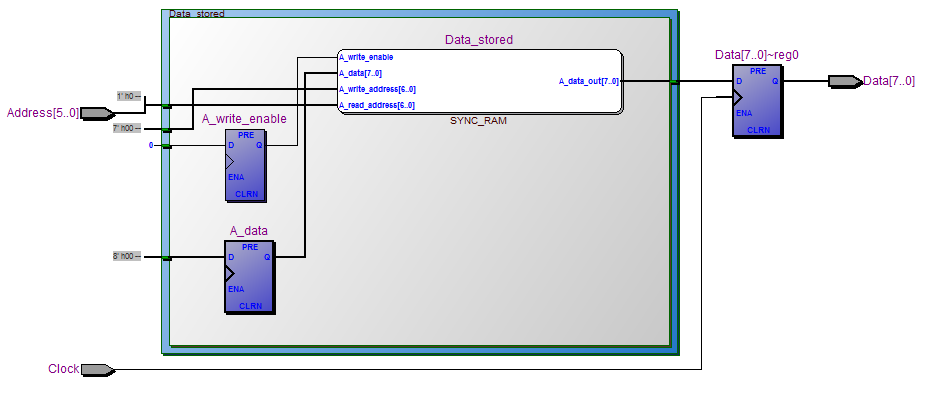
\includegraphics[width=\textwidth]{Figures/ramsynth.png}
\caption{Synthesis of the Program ROM module}
\label{fig:ramsynth}
\end{figure}
